\documentclass{ximera}

%\graphicspath{
  {./}
  {images}        
}
\renewcommand{\d}{\mathop{}\!d}

\title{Steps to create a course Shell }
\begin{document}
\begin{abstract}
\end{abstract}
\maketitle

\section{Create a course repository locally on your computer from Github app}
\begin{enumerate}
\item File/New Repository
\begin{center}
\begin{figure}[h]
<<<<<<< HEAD
\includegraphics[scale=.1]{/images/x1}
=======
\includegraphics[scale=.1]{images/x1}
>>>>>>> f9505e5bb283e3b63a95afc741c2318557d427e5
\end{figure}
\end{center}
\item	Choose path
\item Initialize this with ReadMe
\end{enumerate}

\section{Create ``preamble.tex" and ``main.tex" (need it in every repository)}
\begin{enumerate}
\item Where parts are called (activities)
\begin{center}
\begin{figure}
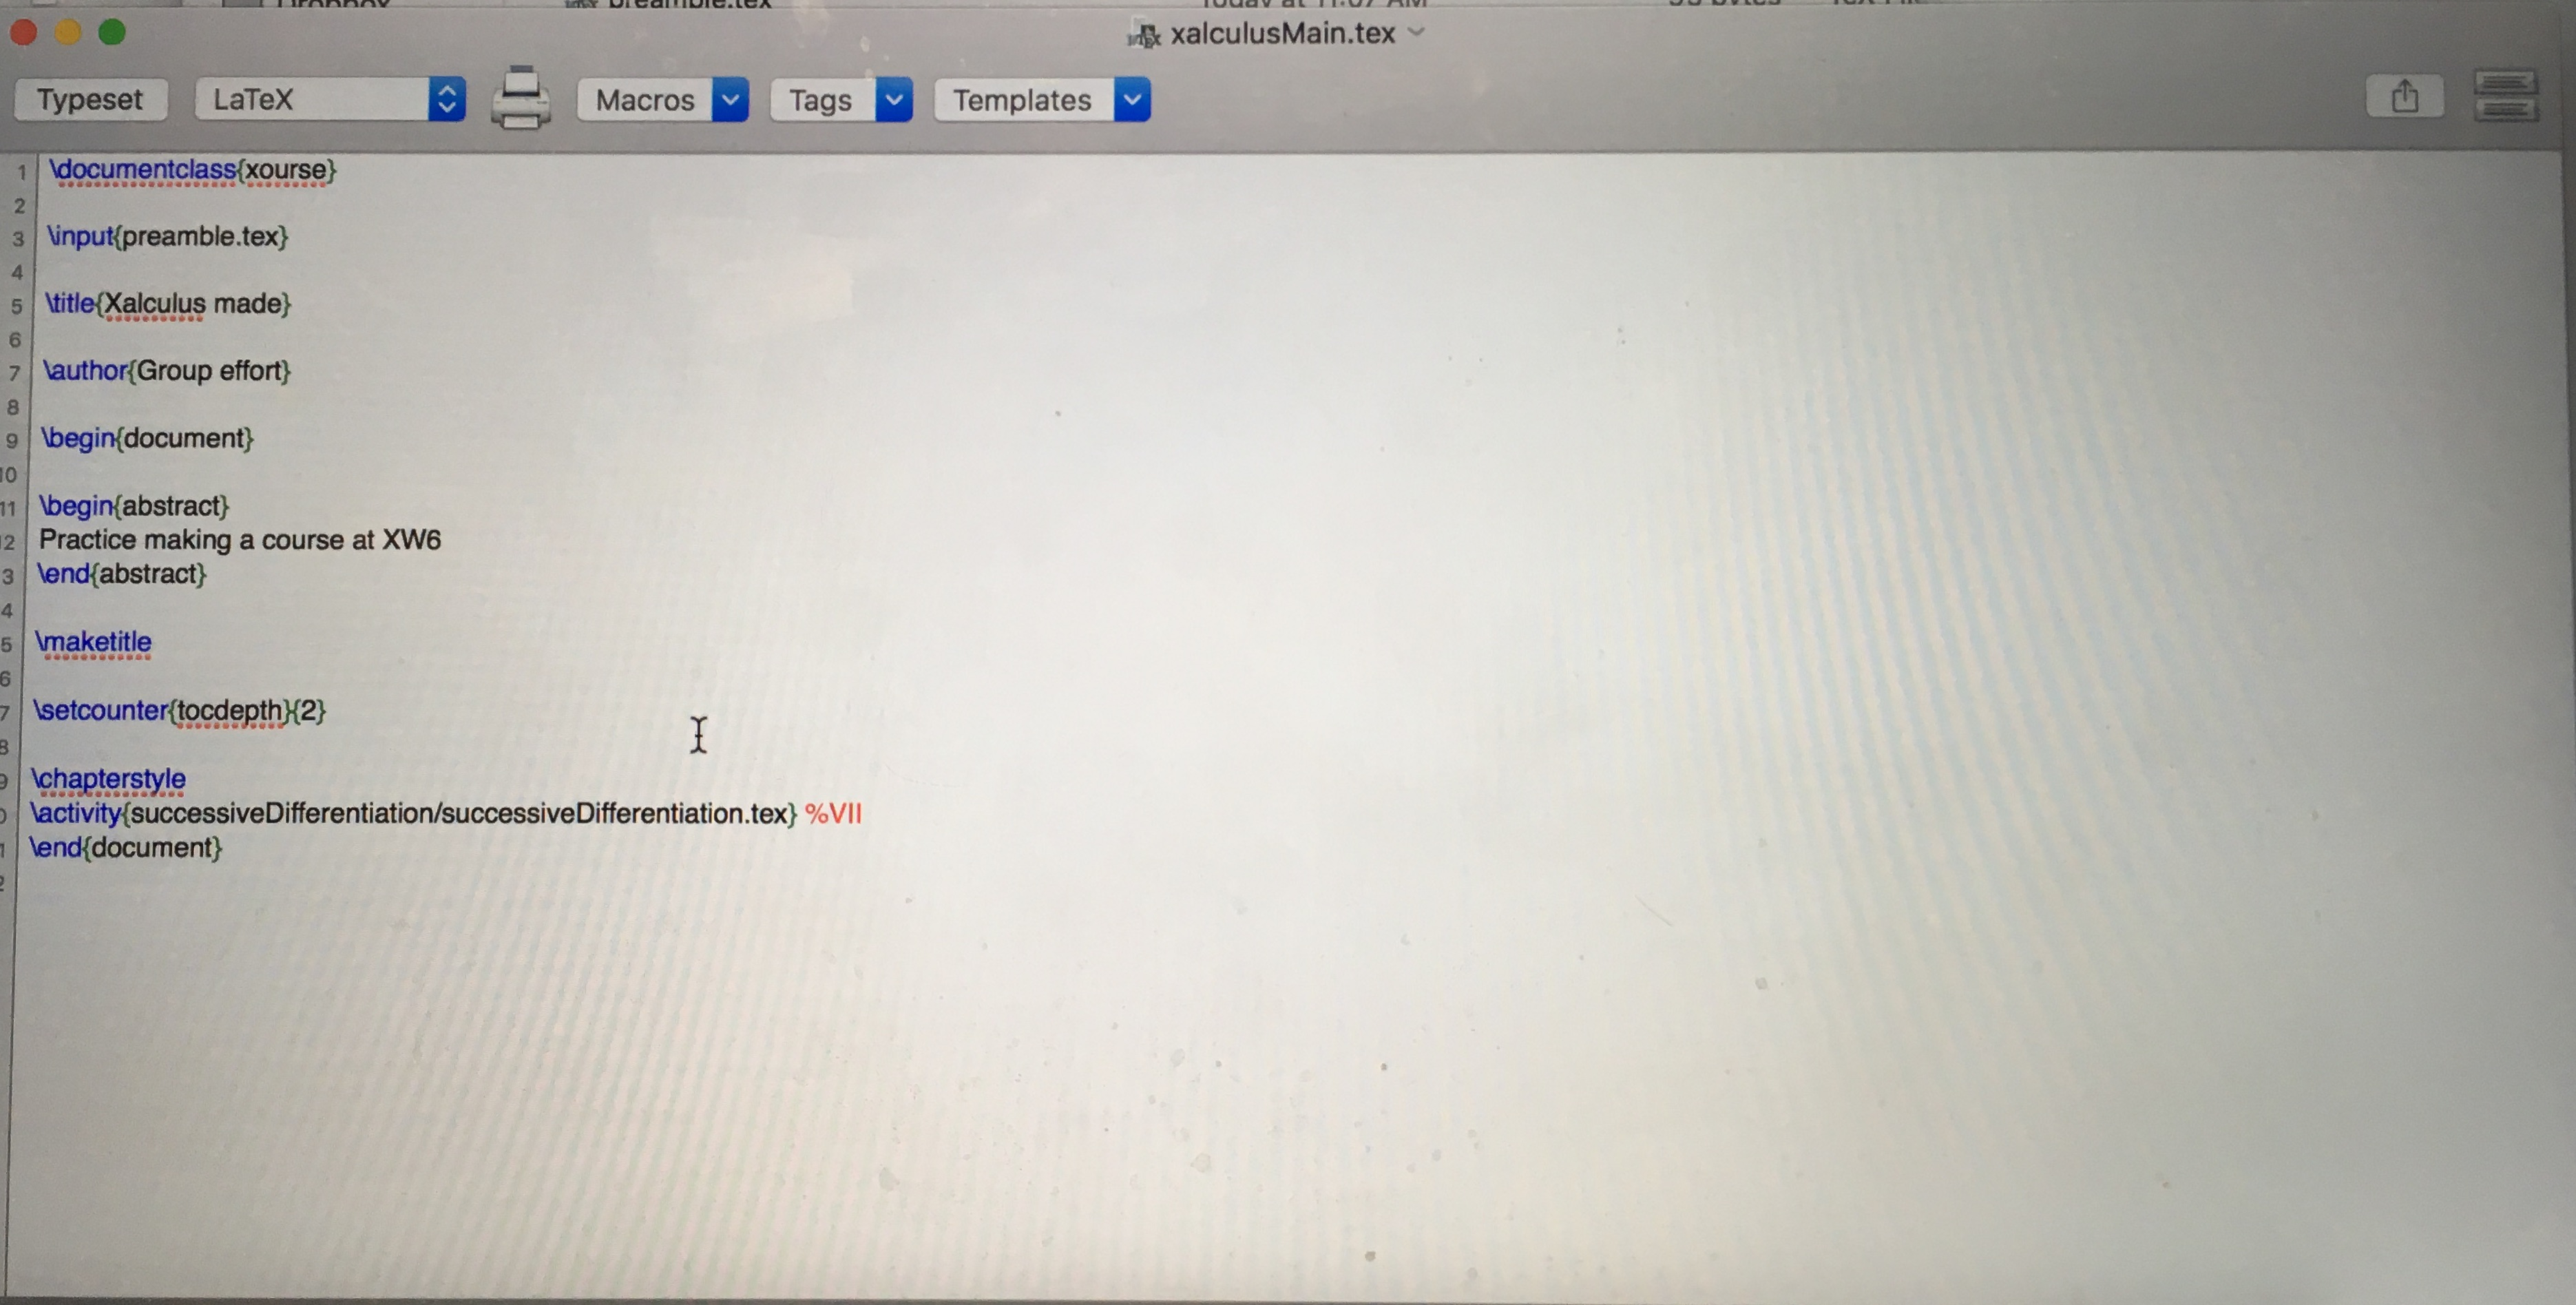
\includegraphics[scale=.07]{images/main}
\end{figure}
\end{center}
\end{enumerate}

\section{Back to app}
\begin{enumerate}
\item Commit to master
\begin{center}
<<<<<<< HEAD
\includegraphics[scale=.09]{/mages/x2}
=======
\includegraphics[scale=.09]{images/x2}
>>>>>>> f9505e5bb283e3b63a95afc741c2318557d427e5
\end{center}
\item Publish repository/publish repository   
\begin{center}
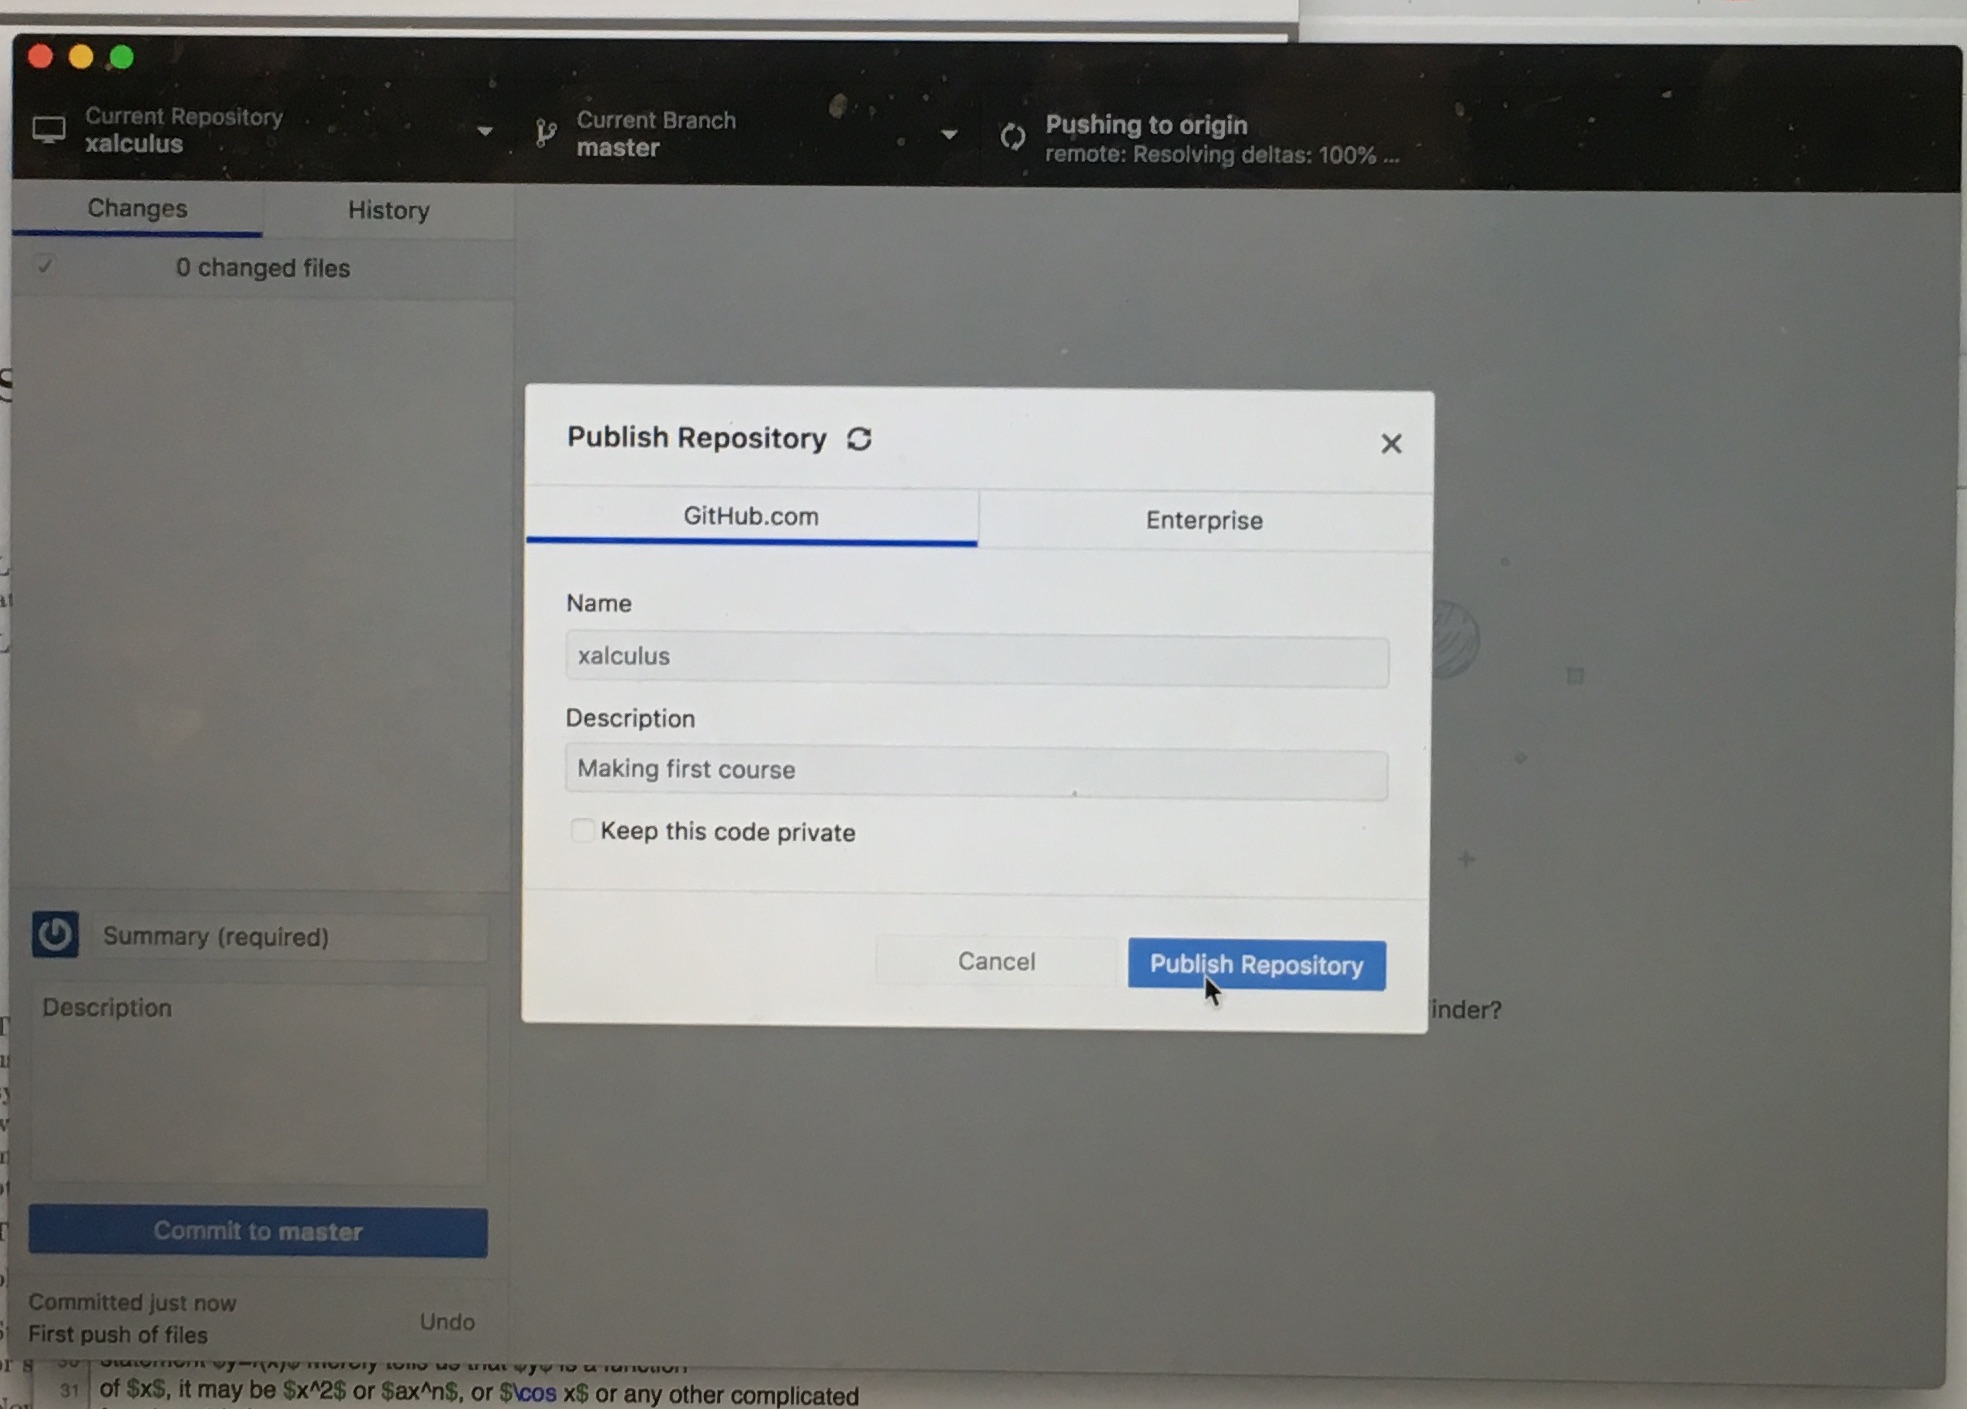
\includegraphics[scale=.09]{images/x3}
\end{center}
\end{enumerate}

\subsection{whenever a change is made to the .tex file we need to push to the repository}
\begin{enumerate}
\item Commit to master
\item Push to origin ***Changes found on the github website
\end{enumerate}

\section{From terminal: (inside repository)}
\begin{enumerate}
\item xake bake
\item	xake frost
\item	xake serve: If first for this course error: remote ximera does not exist,  
\begin{itemize}
\item Run in terminal xake -k YOUR-GPG-KEY name nameOfCourseRepo
\item xake serve again
\end{itemize}
\end{enumerate}

\section{if everything went well: https://ximera.osu.edu/nameOfCourse exists!!!}



\end{document}